
\documentclass[paper=a4, fontsize=11pt]{scrartcl}
\usepackage[T1]{fontenc}
\usepackage{fourier}

\usepackage[english]{babel}															% English language/hyphenation
\usepackage[protrusion=true,expansion=true]{microtype}	
\usepackage{amsmath,amsfonts,amsthm} % Math packages
\usepackage[pdftex]{graphicx}	
\usepackage{url}
\usepackage[margin=1in]{geometry}

%%% Custom sectioning
\usepackage{sectsty}
\allsectionsfont{\centering \normalfont\scshape}


%%% Custom headers/footers (fancyhdr package)
\usepackage{fancyhdr}
\pagestyle{fancyplain}
\fancyhead{}											% No page header
\fancyfoot[L]{}											% Empty 
\fancyfoot[C]{}											% Empty
\fancyfoot[R]{\thepage}									% Pagenumbering
\renewcommand{\headrulewidth}{0pt}			% Remove header underlines
\renewcommand{\footrulewidth}{0pt}				% Remove footer underlines
\setlength{\headheight}{10pt}
\setlength{\headsep}{10pt}
\setlength{\textheight}{700pt}
\setlength{\footskip}{50pt}

%%% Equation and float numbering
\numberwithin{equation}{section}		% Equationnumbering: section.eq#
\numberwithin{figure}{section}			% Figurenumbering: section.fig#
\numberwithin{table}{section}				% Tablenumbering: section.tab#


%%% Maketitle metadata
\newcommand{\horrule}[1]{\rule{\linewidth}{#1}} 	% Horizontal rule

\title{
		\vspace{-3ex}
		\usefont{OT1}{bch}{b}{n}
		\normalfont \normalsize \textsc{School of Computer Science} \\ [25pt]
		\horrule{0.5pt} \\[0.4cm]
		\huge Tiny: Tracking People using Multiple Kinects \\
		\horrule{2pt} \\[0.5cm]
		\vspace{-2ex}
}
\author{
		\normalfont 								\normalsize
        Chi-Jui Wu\\[-3pt]		\normalsize
        \today
}
\date{}

\begin{document}
\maketitle

\section{Project}

People detection and tracking in realtime are essential in personalized robotics, surveillance, interactive systems, and medical monitoring. However, the task of detecting and tracking moving targets in complex scenes is non-trivial. There are many sources of tracking errors, including sensor data noise, occlusion, illumination levels, and cluttered or moving backgrounds. The current project proposes an algorithm for tracking people using multiple Kinects which aim to resolve partial and full occlusion.

\subsection{Contributions}

\subsubsection{Resolve occlusion in one or more Kinects}

Real world environments are complex and unpredictable. Occlusion occurs when the tracked target is hidden by other objects in the field of view of one or more cameras. It increases the difficulty of people detection and tracking. There are two types of occlusions. Static occlusion refers to stationary objects, and it can be accounted by placing cameras at locations that would together capture the entire world view. Dynamic occlusion arises from the interactions of tracked targets in the environment, such as when two people walk past each other. The project aims to resolve both types of occlusion using multiple Kinects. 

The problem is illustrated in Figure \ref{fig:occlusion_problem}. The targets within the image are occluded by the red obstacle, and they are invisible when standing directly in front of the Kinect placed at the top center location. However, the other Kinect on the right hand side is able to detect the targets without any occlusion. The proposed algorithm would use visual and depth sensor information from multiple Kinects to perform people detection and tracking. A new world view would be produced by merging the field of views of the connected Kinects.

\begin{figure}
	\centering
    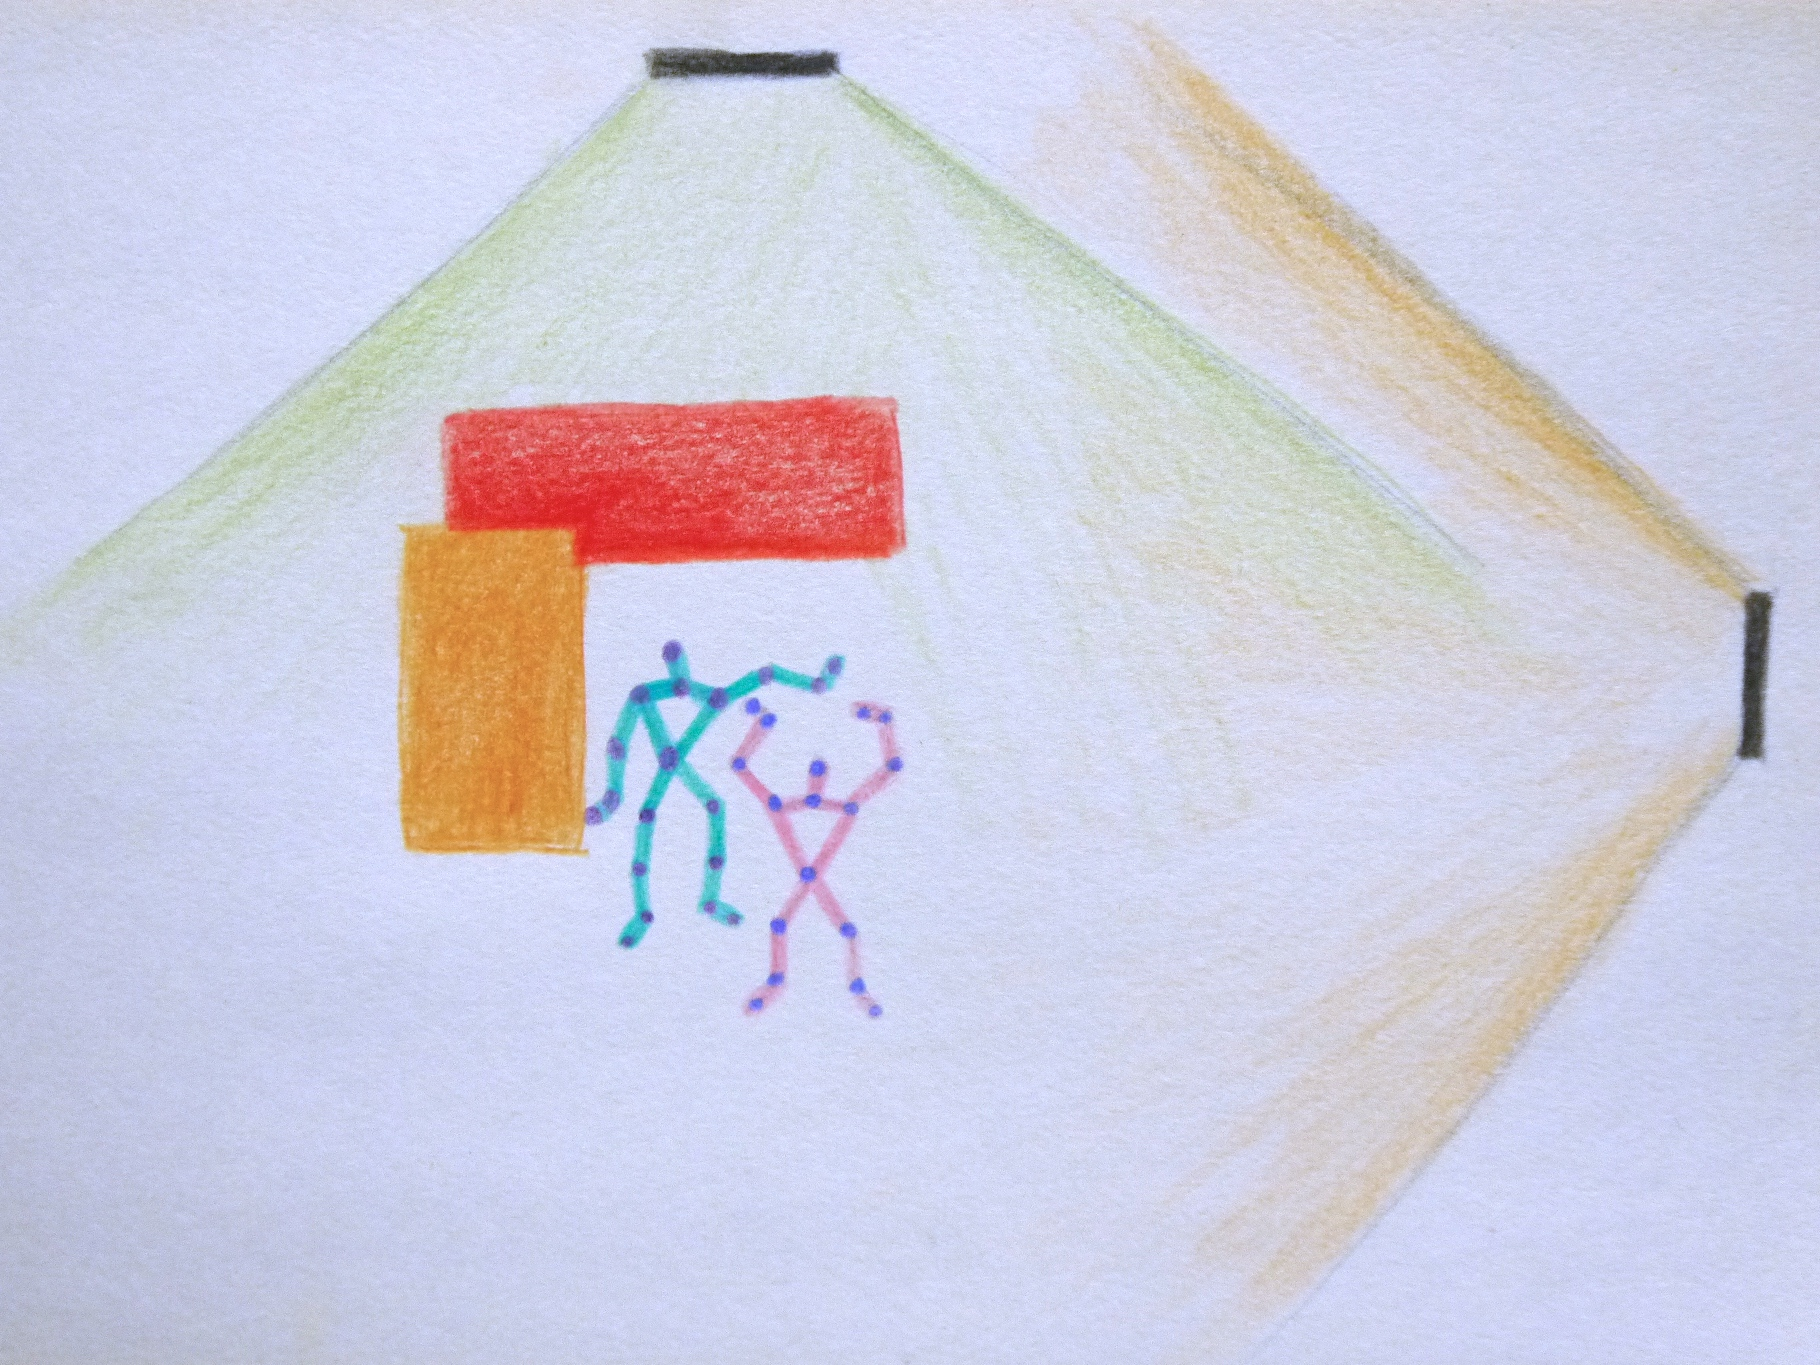
\includegraphics[width=0.8\textwidth]{occlusion}
    \caption{The problem of occlusion}
    \label{fig:occlusion_problem}
\end{figure}

\subsection{Kinect}

Kinect is a low-cost sensor for motion capturing and tracking. The sensor provides infrared, RGB, and depth streams at high frame rates. A hybrid algorithm that uses multiple sensor inputs has the advantage of utilizing relevant visual information for performing a specific task. For instance, depth data is useful for separating a clustered group into sub clusters of individuals, whereas color data is useful for matching a target among visually different people.

\section{Related Work}

This section will review the state of the art techniques in people tracking.

\subsection{Tracking by detection}

Tracking by detection is the primary modern approach to people tracking. The approach leverages the technology of reliable, inexpensive RGB-D sensors, such as the Microsoft Kinect. Person detection has been performed using depth information [12, 13, 14], and with Kinect depth data [18, 19]. Others use only RGB data [1, 15, 16]. Methods using a combination of appearance and depth information also show promising results [5, 17]. 

\subsubsection{RGB-based tracking}

RGB-based tracking consists of methods involving the use of statistical training to produce discriminative appearance models. The models are then used to separate humans from non-human objects. Gavrila et al extract depth features from images and match them against a hierarchy of templates to detect pedestrians in realtime [0]. Mikolajczyk1 et al proposes a human detection method based on robust body part detectors [3]. The method selects local features learned from training examples using Adaptive Boosting, a machine learning technique that gradually improves the model based on the errors of the previous models. Felzenswalb et al proposes a similar method using deformable part based models to detect people in occlusion [20]. Lowe presents the scale-invariant feature transform (SIFT) technique to extract highly distinctive interest points from images that can be used to identify objects from different views [6]. RGB-based tracking can fail to detect people with various poses and when the occlusion is severe.

\subsubsection{Depth-based tracking}

Depth information is important, because people may not have persistence color and texture when they move or interact with others, but they would always occupy a region of space over time. Plagemann et al proposes an interest points detector to identify different body parts in depth images [21]. Ikemura and Fujiyoshi perform people detection using similarity features from local depth histograms[22]. Other discriminative models detect people using directional changes in depth map [5] and incorporating multiple sensor inputs [17].

Xia et al proposes a generative method for people tracking using depth information from the Kinect [19]. Initially, the proposed method uses the nearest neighbor interpolation algorithm to fill missing depth data with similar values to the neighbors. It also applies a median filter on the depth array to smooth the depth pixels. Then, a process known as 2D chamfer distance matching is used to find regions that may contain a person by using edge information in the depth array. The method translate and position a head template to match it against the resulting edge map of the selected regions. A 2-D head contour model and a 3-D head surface models are used to differentiate whether a region is actually a head. The whole body contours are then extracted using a region growing algorithm. This allows the tracked body to be segmented from other objects nearby. Color-based tracking is performed based on the assumption that an object would have similar RGB values in successive time frames. On the other hand, depth-based tracking measures the movements of the objects in 3-D space. The method assume that the coordinates and speed of each detected person change slowly, hence the tracking is performed by matching targets with the least energy scores.

\subsection{Detection techniques using RGB-D}

The following section will survey commonly used techniques in people detection using RGB and depth data.

\subsubsection{Color normalization}

[Paper: Color transfer between images]. The distribution of color values in an image may vary depending on the illumination due to the lighting condition in the environment or the use of different cameras. Color normalization can mitigate this effect. In addition, the normalization process is useful in computing the local color histograms within an image. A local region would be represented by a histogram of visually similar colors. The difference between different local histograms can then be used to match the same object together.

\subsubsection{Color histogram}
A color histogram is the distribution of colors in an image. It represents how many pixels have a particular range of values in the color spaces within an image. Two histograms can be compared using different metrics, such as correlation and intersection. A color histogram based people tracking system is able to keep track of moving people after occlusion and changing illumination [4].  

\subsubsection{HOG: Histogram of Oriented Gradients}

Moreover, Dalal and Bill Triggs show experimentally that Histograms of Oriented Gradient (HOG) descriptors outperform existing human detectors [1]. HOG is one of the most widely used techniques for people detection [7, 8], and subsequent work show that it can not only reliably track similar targets but also increase the performance of tracking algorithm [2, 9, 10].

The method evaluates local histogram of image gradient orientations. An image gradient is a directional change in the color intensity in a fixed-size detection window. Each detection window is divided into cells. A histogram of gradient directions is created for the the pixels within the cell. Local features can be characterized by the distribution of the local gradients. The local histograms of a group of cells, or a block, are normalized. That is, differences among the local histograms of a block are small. The normalization procedure ensures the histograms are invariant to changes in illumination and contrast. HOG is represented as a collection of normalized descriptor blocks, each describing the local features of a region in an image. The descriptor is then used to train a linear Support Vector Machine(SVM) to do person and non-person classification. To detect multiple people, the detection window is scrolled over the image at different scales and the corresponding descriptors are computed to train the SVM.

\subsubsection{HOD: Histogram of Oriented Depths}

Inspired by HOG, Spinello and Arras develop a person detector called Histogram of Oriented Depths (HOD) for dense depth data [5]. Similarly to HOG, HOD divides a fixed-size detection window into cells. Instead of encoding changes in color intensity, it computes the local oriented depth gradients and creates a histogram for each cell. The histograms of a block, or four cells, are normalized. HOG captures local 2D shape, whereas HOD captures local 3D shape. The descriptors are also taken for training a linear SVM. HOD uses the depth information to make an informed scale-space search, as opposed to the uninformed search in the HOG approach. Thus, this method uses a smaller number of detection window scales, thus reducing the computational cost.

\subsubsection{Combo-HOD: RGB-D people detector}

Spinello and Arras propose a novel person detector that probabilistically combines HOG and HOD [5]. HOG uses image data which are rich in color and texture but poor under changing illumination, and HOD uses depth data which are invariant to illumination changes. Combo-HOD trains a HOG detector on image data and a HOD detector on depth data. The method relies on the informed scale-space search which uses HOD descriptors and HOG descriptors on the same detection window at scales that are compatible with the presence of people in the image. [Need to read the papers again]

The Kinect depth information becomes highly unreliable over eight meters from the sensor; however, using a combined approach of HOG and HOD can increase the reliability of the overall tracking algorithm. The method does not rely background segmentation nor a ground plane assumption, but it relies on heavy GPU implementation. [Discuss more results]

\subsubsection{Tracking within groups}

Munaro et al propose a depth-based sub-clustering method for detecting and tracking people within groups [10]. The method can detect people with dynamic occlusion, such as when people are standing very close or walking past each other. The tracking algorithm performs the detection and tracking association using motion, appearance, and detection confidence. An online learned classifier is also used to track people by learning negative examples from the detection process.

The proposed method consists of a voxel grid filtering procedure which reduces the size of the RGB-D point cloud for processing. It divides the depth space into voxels, where each voxel contains sample depth values that are some distance apart. A height map is obtained for each cluster using depth information, and sub-clusters are created by finding the local maxima within the height map. A bounding box is made for each cluster, where its boundary should contain a person's whole body. Then, the method applies a HOG detector to the bounding box of each sub-cluster.

For every tracked sub-cluster, a RGB color histogram is computed. The appearance of each tracked target is learned via an online classifier. The tracking module formulates the detection and tracking association [TODO].

The algorithm runs at 26 frames per second and does not involve a GPU implementation.

\subsection{More papers}

Robust Tracking-by-Detection using a Detector Confidence Particle Filter

Detecting and Tracking People using an RGB-D Camera via Multiple Detector
Fusion

Real-Time Multi-Person Tracking with Detector Assisted Structure Propagation

Human Detection with Occlusion Handling by Over-Segmentation and Clustering on Foreground Regions

3D flow estimation for human action recognition from colored point clouds

\subsection{Multiple Kinects}

\subsubsection{Calibration}

\subsubsection{Merging the FOVs}

\subsubsection{Scheduling}

Intelligent sensor-scheduling for multi-kinect-tracking

\section{Current Approach}

\section{References}

[0] Vision-Based Pedestrian Detection: The PROTECTOR System

[1] Histograms of Oriented Gradients for Human Detection

[2] Exploring Context Information for Inter-Camera Multiple Target Tracking

[3] Human Detection Based on a Probabilistic Assembly of Robust Part Detectors

[4] A COLOR HISTOGRAM BASED PEOPLE TRACKING SYSTEM

[5] People Detection in RGB-D Data

[6] Distinctive Image Features from Scale-Invariant Keypoints

[7] Pedestrian detection: A benchmark

[8] Monocular pedestrian detection: Survey and experiments

[9] People tracking in RGB-D data with on-line boosted target models

[10] Tracking people within groups with RGB-D data

[11] Detecting pedestrians using patterns of motion and appearance

[12] Human detection using depth and gray images

[13] Multi-cue pedestrian detection and tracking from a moving vehicle

[14] Real-Time Human Detection Using Relational Depth Similarity Features

[15] Robust tracking-by-detection using a detector confidence particle filter

[16] Rapid object detection using a boosted cascadeof simple features

[17] Detecting and tracking people using an rgb-d camera via multiple detector fusion

[18] A system for change detection and human recognition in voxel space using the microsoft kinect sensor

[19] Human detection using depth information by kinect

[20] Object detection with discriminatively trained part-based models

[21] Realtime identification and localization of body parts from depth images
\end{document}
